\documentclass[12pt]{article}
\usepackage{amsmath}
\usepackage{graphicx}
\usepackage{amsfonts}
\usepackage{float}
\usepackage{geometry}
\geometry{a4paper, margin=1in}

\documentclass[12pt]{article}
\usepackage{amsmath}
\usepackage{graphicx}
\usepackage{amsfonts}
\usepackage{float}
\usepackage{geometry}
\geometry{a4paper, margin=1in}

\title{Kinodynamic Path Planning and Control in Robotics Using RRT and PID}
\author{Mark Doughten, Shubham Patil, Vijayendra Sai Chennareddy}
\date{\today}

\begin{document}

\maketitle

\section{Introduction}
In robotics, autonomous path planning and control are crucial aspects of robot navigation, particularly in environments with obstacles. The objective of this project is impementing a hybrid approach that combines kinodynamic Rapidly-exploring Random Tree (RRT) for path planning and Proportional-Integral-Derivative (PID) controllers for executing the motion along the planned path. This work is demonstrated using a ball in a MuJoCo simulation environment, where the ball navigates through an environment containing walls and boundaries. The goal is moving the ball from a starting position to a goal position while avoiding obstacles using the kinodynamic RRT algorithm and accurately controlling the movement with PID.

\subsection{Objectives}
The main challenge is efficiently generating a collision-free path from a start point to a goal point in a cluttered environment and ensure the ball follows this path with minimal deviation. We took the following steps to achieve the objective.
\begin{itemize}
    \item Implement a Trapezoidal decomposition (\(\mathcal{C} = \mathbb{R}^3_{\text{max}}\)) plan a path in a 3D environment with a rectangular obstacle.

    \begin{figure}[h!]
      \centering
      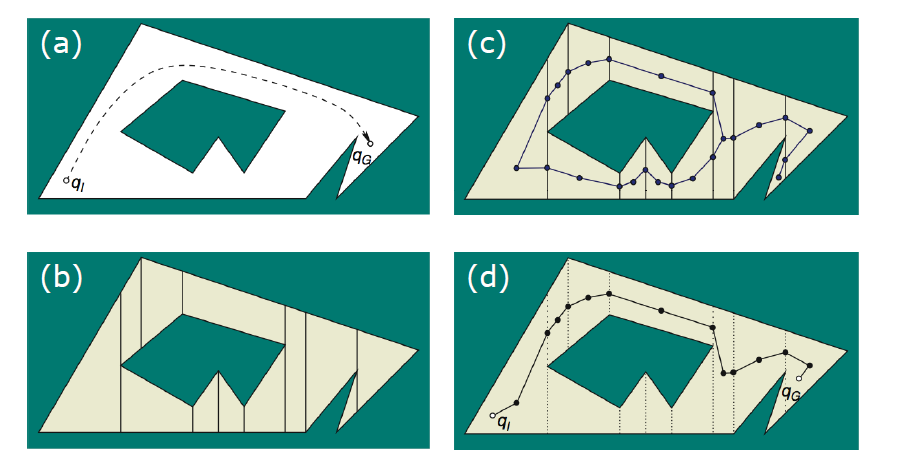
\includegraphics[width=0.5\textwidth]{/images/trapezoidal.png}
      \caption{This is the caption of the image.}
      \label{fig:sample_image}
    \end{figure}

    
    \item Implement a Trapezoidal decomposition (\(\mathcal{C} = \mathbb{R}^3_{\text{max}}\)) plan a path in a 3D environment with a rectangular obstacle.
    
    \item Use PID controllers to control the robot's movement to follow the planned path.
    \item Simulate the robot's movement in the MuJoCo physics engine and visualize the results.
    \item Implement kinodynamic RRT to plan a path in a 2D environment with obstacles.
    \item Use PID controllers to control the robot's movement to follow the planned path.
    \item Simulate the robot's movement in the MuJoCo physics engine and visualize the results.
\end{itemize}

\section{Environment Setup}
The environment consists of a 2D plane with predefined walls and boundaries. The simulation is conducted using the MuJoCo physics engine, which allows the creation and control of dynamic models. For this project, a ball is used as the robot, and it is moved through the environment containing a set of obstacles. The model used is defined in the \texttt{ball\_square.xml} file, and the walls are represented as both external boundaries and internal obstacles.

\subsection{Map Description}
\begin{itemize}
    \item \textbf{Dimensions:} The 2D environment spans from $x = -0.5$ to $x = 1.5$ and $y = -0.4$ to $y = 0.4$.
    \item \textbf{Obstacles:} A rectangular obstacle is placed in the middle of the environment between coordinates (0.5, -0.15) and (0.6, 0.15), acting as a wall.
    \item \textbf{Goal Area:} The target area for the robot is set between coordinates (0.9, -0.3) and (1.1, 0.3).
    \item \textbf{Boundaries:} The outer walls of the environment prevent the robot from moving outside the area.
\end{itemize}
This setup ensures the presence of both static and dynamic constraints, making path planning non-trivial and control challenging.

\section{Kinodynamic RRT for Path Planning}

\subsection{Algorithm Overview}
Rapidly-exploring Random Trees (RRT) are widely used for motion planning in high-dimensional spaces. In this project, a kinodynamic variant of RRT is implemented. Unlike standard RRT, kinodynamic RRT accounts for the robot’s dynamics while generating the tree, ensuring that the planned path can be followed realistically by the robot. This approach helps in avoiding sharp or unrealistic turns that the robot may not be able to follow.

The algorithm grows a tree from the start position by:
\begin{enumerate}
    \item Sampling a random point in the environment.
    \item Identifying the nearest node in the tree.
    \item Applying a control input to move the robot towards the sampled point, simulating its dynamics.
    \item Checking the resulting position for collisions.
    \item Adding the new position to the tree if no collision occurs.
\end{enumerate}

This process repeats until the robot reaches the goal area or a maximum number of iterations is reached. The function \texttt{kinodynamic\_rrt} implements this process, and \texttt{simulate} handles the forward simulation of the robot’s dynamics.

\subsection{Collision Avoidance}
Collision detection is handled by the function \texttt{is\_collision\_free}, which checks if the robot’s new position lies within any of the obstacle regions or the environment boundaries. A safety margin is applied to ensure that the robot does not approach obstacles too closely.

\subsection{Path Construction}
If the algorithm successfully finds a path to the goal, the tree is traversed back from the goal node to the start node to construct the path. The function \texttt{construct\_path} handles this backtracking. Finally, the path is visualized using \texttt{plot\_path\_with\_boundaries\_and\_mixed\_obstacles}, which shows the path, the environment boundaries, and the obstacles.

\section{PID Control for Path Following}

\subsection{PID Controller Overview}
Proportional-Integral-Derivative (PID) controllers are commonly used in control systems to achieve stable and accurate control. In this project, two PID controllers are implemented: one for controlling the movement of the ball in the $x$-direction and the other for the $y$-direction. Each controller computes the control input based on the error between the current and target positions, aiming to reduce this error over time.

The function \texttt{move\_ball\_to\_position\_with\_pid} implements the control loop, where the ball’s current position is compared to the target position from the planned path. The PID controllers compute the necessary force to move the ball toward the target, and the control inputs are applied in each iteration of the simulation.

\subsection{Tuning of PID Gains}
The gains for the PID controllers were manually tuned to achieve smooth movement without overshooting. The proportional (\texttt{kp}), integral (\texttt{ki}), and derivative (\texttt{kd}) gains were set as follows:
\begin{itemize}
    \item \textbf{Proportional Gain (kp):} 0.1 — provides a basic correction based on the current error.
    \item \textbf{Integral Gain (ki):} 0 — was not used in this implementation to avoid cumulative errors from drift.
    \item \textbf{Derivative Gain (kd):} 0.4 — helps to smooth the response by anticipating future errors based on the rate of change.
\end{itemize}

\subsection{Path Following}
The PID controllers move the ball sequentially through each waypoint in the planned path. The movement is clamped to prevent overshooting, and the simulation continues until the ball reaches the goal position with minimal error (set to 0.05 in this case).

\subsection{Control Challenges}
Some challenges in the control process included handling sharp turns in the path and adjusting the control parameters to prevent oscillations. The derivative gain played a crucial role in damping the response and ensuring smooth transitions between waypoints.

\section{Conclusion}
This project successfully integrated kinodynamic RRT for path planning and PID control for path execution in a simulated 2D environment. By leveraging these techniques, the robot (ball) was able to navigate a complex environment with obstacles and boundaries while accurately following the planned path to the goal.

\end{document}
